
%% Vectors and Motion Questions used on the
%% NYSED Physics Regents Examination
%%--------------------------------------------------

%% this section contains 68 problems


%% Section June2015
%%--------------------
\element{nysed}{
\begin{question}{June2015-Q01}
    Which quantities are scalar?
    \begin{choices}
      \correctchoice{speed and work}
        \wrongchoice{velocity and force}
        \wrongchoice{distance and acceleration}
        \wrongchoice{momentum and power}
    \end{choices}
\end{question}
}

\element{nysed}{
\begin{question}{June2015-Q03}
    An airplane traveling north at \SI{220}{\meter\per\second} encounters a \SI{50.0}{\meter\per\second} crosswind from west to east,
        as represented in the diagram below.
    \begin{center}
        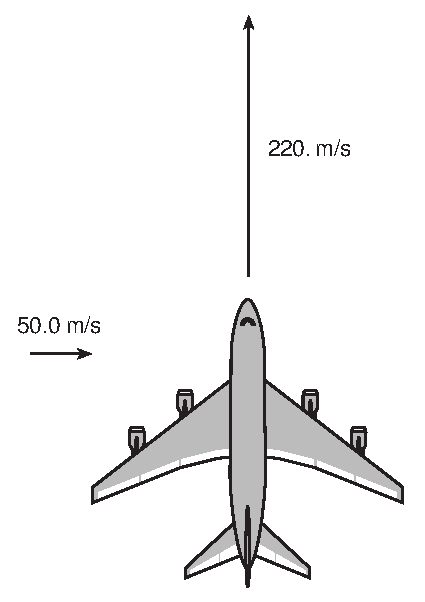
\includegraphics[keepaspectratio,scale=0.95]{June2015-Q03}
    \end{center}
    What is the resultant speed of the plane?
    \begin{multicols}{2}
    \begin{choices}
        \wrongchoice{\SI{170}{\meter\per\second}}
        \wrongchoice{\SI{214}{\meter\per\second}}
      \correctchoice{\SI{226}{\meter\per\second}}
        \wrongchoice{\SI{270}{\meter\per\second}}
    \end{choices}
    \end{multicols}
\end{question}
}

\element{nysed}{
\begin{question}{June2015-Q37}
    The vector diagram below represents the velocity of a car traveling \SI{24}{\meter\per\second} \ang{35} east of north.
    \begin{center}
    \begin{tikzpicture}
        \draw[dashed] (-1,0) -- (2,0) node[pos=0,anchor=east] {W} node[pos=1,anchor=west] {E};
        \draw[dashed] (0,-1) -- (0,2) node[pos=0,anchor=north] {S} node[pos=1,anchor=south] {N};
        \draw[thick,->] (0,0) -- ++(55:2.0cm);
        \draw[] (55:1.0cm) arc (55:90:1.0cm) node[pos=0.5,anchor=south,font=\small] {\ang{35}};
    \end{tikzpicture}
    \end{center}
    What is the magnitude of the component of the car's velocity that is directed eastward?
    \begin{multicols}{2}
    \begin{choices}
      \correctchoice{\SI{14}{\meter\per\second}}
        \wrongchoice{\SI{20}{\meter\per\second}}
        \wrongchoice{\SI{29}{\meter\per\second}}
        \wrongchoice{\SI{42}{\meter\per\second}}
    \end{choices}
    \end{multicols}
\end{question}
}


%% Section June2014
%%--------------------
\element{nysed}{
\begin{question}{June2014-Q01}
    Which quantity is scalar?
    \begin{multicols}{2}
    \begin{choices}
      \correctchoice{mass}
        \wrongchoice{force}
        \wrongchoice{momentum}
        \wrongchoice{acceleration}
    \end{choices}
    \end{multicols}
\end{question}
}

\element{nysed}{
\begin{question}{June2014-Q03}
    The components of a \SI{15}{\meter\per\second} velocity at an angle of \ang{60} above the horizontal are:
    \begin{choices}
      \correctchoice{\SI{13}{\meter\per\second} vertical and \SI{7.5}{\meter\per\second} horizontal}
        \wrongchoice{\SI{7.5}{\meter\per\second} vertical and \SI{13}{\meter\per\second} horizontal}
        \wrongchoice{\SI{6.0}{\meter\per\second} vertical and \SI{9.0}{\meter\per\second} horizontal}
        \wrongchoice{\SI{9.0}{\meter\per\second} vertical and \SI{6.0}{\meter\per\second} horizontal}
    \end{choices}
\end{question}
}


%% Section June2013
%%--------------------
\element{nysed}{
\begin{question}{June2013-Q02}
    Two \SI{20}{\newton} forces act concurrently on an object.
    What angle between these forces will produce a resultant force with the greatest magnitude?
    \begin{multicols}{4}
    \begin{choices}
      \correctchoice{\ang{0}}
        \wrongchoice{\ang{45}}
        \wrongchoice{\ang{90}}
        \wrongchoice{\ang{180}}
    \end{choices}
    \end{multicols}
\end{question}
}


%% Section June2012
%%--------------------
\element{nysed}{
\begin{question}{June2012-Q03}
    A baseball is thrown at an angle of \SI{40.0} above the horizontal.
    The horizontal component of the baseball's initial velocity is \SI{12.0}{\meter\per\second}.
    What is the magnitude of the ball's initial velocity?
    \begin{multicols}{2}
    \begin{choices}
        \wrongchoice{\SI{7.71}{\meter\per\second}}
        \wrongchoice{\SI{9.20}{\meter\per\second}}
      \correctchoice{\SI{15.7}{\meter\per\second}}
        \wrongchoice{\SI{18.7}{\meter\per\second}}
    \end{choices}
    \end{multicols}
\end{question}
}


%% Section June2011
%%--------------------
\element{nysed}{
\begin{question}{June2011-Q01}
    Scalar is to vector as:
    \begin{choices}
      \correctchoice{speed is to velocity}
        \wrongchoice{displacement is to distance}
        \wrongchoice{displacement is to velocity}
        \wrongchoice{speed is to distance}
    \end{choices}
\end{question}
}


%% Section June2010
%%--------------------
\element{nysed}{
\begin{question}{June2010-Q02}
    A motorboat, which has a speed of \SI{5.0}{\meter\per\second} in still water,
        is headed east as it crosses a river flowing south at \SI{3.3}{\meter\per\second}.
    What is the magnitude of the boat's resultant velocity with respect to the starting point?
    \begin{multicols}{2}
    \begin{choices}
        \wrongchoice{\SI{3.3}{\meter\per\second}}
        \wrongchoice{\SI{6.0}{\meter\per\second}}
      \correctchoice{\SI{5.0}{\meter\per\second}}
        \wrongchoice{\SI{8.3}{\meter\per\second}}
    \end{choices}
    \end{multicols}
\end{question}
}


%% Section June2009
%%--------------------
\element{nysed}{
\begin{question}{June2009-Q02}
    The vector diagram below represents the horizontal component, $F_H$,
        and the vertical component, $F_V$, of a \SI{24}{\newton} force acting at \ang{35} above the horizontal.
    \begin{center}
    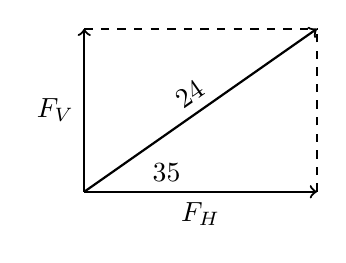
\begin{tikzpicture}[scale=1.5]
        \draw[thick,->] (0,0) -- (0,1.38) node[pos=0.5,anchor=east] {$F_V$};
        \draw[thick,->] (0,0) -- (1.97,0) node[pos=0.5,anchor=north] {$F_H$} node[pos=0.25,anchor=south west] {\ang{35}};
        \draw[thick,dashed] (0,1.38) -- (1.97,1.38);
        \draw[thick,dashed] (1.97,0) -- (1.97,1.38);
        \draw[thick,->] (0,0) -- (1.97,1.38) node[pos=0.5,anchor=south,rotate=35] {\SI{24}{\newton}};
    \end{tikzpicture}
    \end{center}
    What are the magnitudes of the horizontal and vertical components?
    \begin{choices}
        \wrongchoice{$F_H=\SI{3.5}{\newton}$ and $F_V=\SI{4.9}{\newton}$}
        \wrongchoice{$F_H=\SI{4.9}{\newton}$ and $F_V=\SI{3.5}{\newton}$}
        \wrongchoice{$F_H=\SI{14}{\newton}$ and $F_V=\SI{20.}{\newton}$}
      \correctchoice{$F_H=\SI{20.}{\newton}$ and $F_V=\SI{14}{\newton}$}
    \end{choices}
\end{question}
}


%% Section June2008
%%--------------------
\element{nysed}{
\begin{question}{June2008-Q01}
    The speedometer in a car does \emph{not} measure the car's velocity because velocity is a:
    \begin{choices}
      \correctchoice{vector quantity and has a direction associated with it}
        \wrongchoice{vector quantity and does not have a direction associated with it}
        \wrongchoice{scalar quantity and has a direction associated with it}
        \wrongchoice{scalar quantity and does not has a direction associated with it}
    \end{choices}
\end{question}
}

\element{nysed}{
\begin{question}{June2008-Q11}
    An airplane flies with a velocity of \SI{750}{\kilo\meter\per\hour},
        \ang{30} south of east.
    What is the magnitude of the eastward component of the plane's velocity?
    \begin{multicols}{2}
    \begin{choices}
        \wrongchoice{\SI{866}{\kilo\meter\per\hour}}
      \correctchoice{\SI{650}{\kilo\meter\per\hour}}
        \wrongchoice{\SI{433}{\kilo\meter\per\hour}}
        \wrongchoice{\SI{375}{\kilo\meter\per\hour}}
    \end{choices}
    \end{multicols}
\end{question}
}

\element{nysed}{
\begin{question}{June2008-Q41}
    The diagram below represents two concurrent forces.
    \begin{center}
    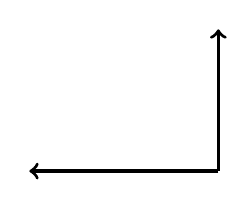
\begin{tikzpicture}[scale=0.60]
        \draw[very thick,->] (0,0) -- (0,3);
        \draw[very thick,->] (0,0) -- (-4,0);
    \end{tikzpicture}
    \end{center}
    Which vector represents the force that will produce equilibrium with these two forces?
    \begin{multicols}{2}
    \begin{choices}
        \AMCboxDimensions{down=-0.9cm}
        \wrongchoice{
            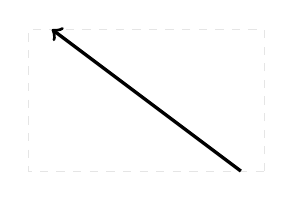
\begin{tikzpicture}[scale=0.60]
                \draw[dashed,white!90!black] (0.5,0) rectangle (-4.5,3);
                \draw[very thick,->] (0,0) -- (-4,3);
            \end{tikzpicture}
        }
        \wrongchoice{
            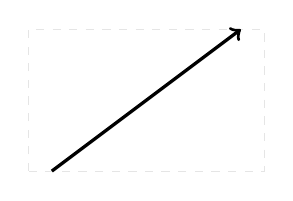
\begin{tikzpicture}[scale=0.60]
                \draw[dashed,white!90!black] (-0.5,0) rectangle (4.5,3);
                \draw[very thick,->] (0,0) -- (4,3);
            \end{tikzpicture}
        }
        %% ANS is 3
        \correctchoice{
            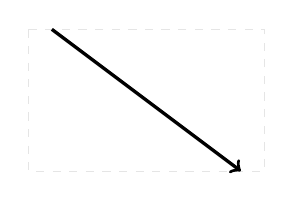
\begin{tikzpicture}[scale=0.60]
                \draw[dashed,white!90!black] (-0.5,0) rectangle (4.5,-3);
                \draw[very thick,->] (0,0) -- (4,-3);
            \end{tikzpicture}
        }
        \wrongchoice{
            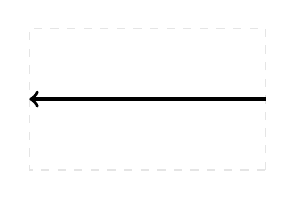
\begin{tikzpicture}[scale=0.60]
                \draw[dashed,white!90!black] (0,-1.5) rectangle (-5,1.5);
                \draw[very thick,->] (0,0) -- (-5,0);
            \end{tikzpicture}
        }
    \end{choices}
    \end{multicols}
\end{question}
}


%% Section Jan2008
%%--------------------
\element{nysed}{
\begin{question}{Jan2008-Q01}
    Which is a vector quantity?
    \begin{multicols}{2}
    \begin{choices}
        \wrongchoice{speed}
        \wrongchoice{mass}
        \wrongchoice{work}
      \correctchoice{displacement}
    \end{choices}
    \end{multicols}
\end{question}
}

\element{nysed}{
\begin{question}{Jan2008-Q04}
    A soccer player kicks a ball with an initial velocity
        of \SI{10}{\meter\per\second} at an angle of
        \ang{30} above the horizontal.
    The magnitude of the horizontal component of the ball's
        initial velocity is:
    \begin{multicols}{2}
    \begin{choices}
      \correctchoice{\SI{8.7}{\meter\per\second}}
        \wrongchoice{\SI{5.0}{\meter\per\second}}
        \wrongchoice{\SI{9.8}{\meter\per\second}}
        \wrongchoice{\SI{10}{\meter\per\second}}
    \end{choices}
    \end{multicols}
\end{question}
}

\element{nysed}{
\begin{question}{Jan2008-Q38}
    Two forces act concurrently on an object.
    Their resultant force has the largest magnitude when
        the angle between the forces is:
    \begin{multicols}{2}
    \begin{choices}
      \correctchoice{\ang{0}}
        \wrongchoice{\ang{90}}
        \wrongchoice{\ang{30}}
        \wrongchoice{\ang{180}}
    \end{choices}
    \end{multicols}
\end{question}
}


%% Section June2007
%%--------------------
\element{nysed}{
\begin{question}{June2007-Q05}
    As the angle between two concurrent forces decreases,
        the magnitude of the force required to produce equilibrium
    \begin{multicols}{2}
    \begin{choices}
        \wrongchoice{decreases}
      \correctchoice{increases}
        \wrongchoice{remains the same}
    \end{choices}
    \end{multicols}
\end{question}
}

\element{nysed}{
\begin{question}{June2007-Q06}
    A child walks \SI{5.0}{\meter} north, then \SI{4.0}{\meter} east,
        and finally \SI{2.0}{\meter} south.
    What is the magnitude of the resultant displacement of the child after
        the entire walk?
    \begin{multicols}{2}
    \begin{choices}
      \correctchoice{\SI{5.0}{\meter}}
        \wrongchoice{\SI{1.0}{\meter}}
        \wrongchoice{\SI{3.0}{\meter}}
        \wrongchoice{\SI{11.0}{\meter}}
    \end{choices}
    \end{multicols}
\end{question}
}

\element{nysed}{
\begin{question}{June2007-Q38}
    A stream is \SI{30}{\meter} wide and it current flows southward at
        \SI{1.5}{\meter\per\second}.
    A toy boat is launched with a velocity of
        \SI{2.0}{\meter\per\second} eastward from the west bank of the stream.
    What is the magnitude of the boat's resultant velocity as it crossed the stream?
    \begin{multicols}{2}
    \begin{choices}
        \wrongchoice{\SI{0.5}{\meter\per\second}}
      \correctchoice{\SI{2.5}{\meter\per\second}}
        \wrongchoice{\SI{3.0}{\meter\per\second}}
        \wrongchoice{\SI{3.5}{\meter\per\second}}
    \end{choices}
    \end{multicols}
\end{question}
}

\element{nysed}{
\begin{question}{June2007-Q39}
    A stream is \SI{30}{\meter} wide and it current flows southward at
        \SI{1.5}{\meter\per\second}.
    A toy boat is launched with a velocity of \SI{2.0}{\meter\per\second}
        eastward from the west bank of the stream.
    How much time is required for the boat to reach the opposite
        bank of the stream?
    \begin{multicols}{2}
    \begin{choices}
        \wrongchoice{\SI{8.6}{\second}}
        \wrongchoice{\SI{12}{\second}}
      \correctchoice{\SI{15}{\second}}
        \wrongchoice{\SI{60}{\second}}
    \end{choices}
    \end{multicols}
\end{question}
}

%% Section Jan2007
%%--------------------
\element{nysed}{
\begin{question}{Jan2007-Q02}
    A \SI{6.0}{\newton} force and an \SI{8.0}{\newton} force act
        concurrently on a point.
    As the angle between these forces increases from \ang{0} to \ang{90},
        the magnitude of their resultant:
    \begin{choices}
      \correctchoice{decreases}
        \wrongchoice{increases}
        \wrongchoice{remains the same}
    \end{choices}
\end{question}
}


%% Section June2006
%%--------------------
\element{nysed}{
\begin{question}{June2006-Q03}
    The diagram below represents a force vector, $A$, and a
        resultant vector, $R$.
    \begin{center}
        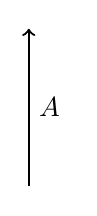
\begin{tikzpicture}
            \draw[thick,->] (0,0) -- (0,2cm);
            \node[thick,anchor=west] at (0,1cm) {$A$};
        \end{tikzpicture}
        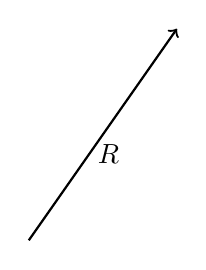
\begin{tikzpicture}
            \draw[thick,->] (0,0) -- (55:3.28cm);
            \node[thick,anchor=north,xshift=2pt] at (55:1.64cm) {$R$};
        \end{tikzpicture}
    \end{center}
    Which force vector $B$ below could be added to force vector
        $A$ to produce resultant vector $R$?
    \begin{multicols}{2}
    \begin{choices}
        \AMCboxDimensions{down=-1.0em}
        \correctchoice{
            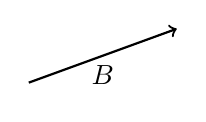
\begin{tikzpicture}
                \draw[thick,->] (0,0) -- (20:2cm);
                \node[thick,anchor=north] at (20:1cm) {$B$};
            \end{tikzpicture}
        }
        \wrongchoice{
            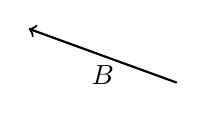
\begin{tikzpicture}
                \draw[thick,->] (0,0) -- (160:2cm);
                \node[thick,anchor=north] at (160:1cm) {$B$};
            \end{tikzpicture}
        }
        \wrongchoice{
            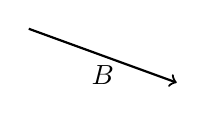
\begin{tikzpicture}
                \draw[thick,->] (0,0) -- (-20:2cm);
                \node[thick,anchor=north] at (-20:1cm) {$B$};
            \end{tikzpicture}
        }
        \wrongchoice{
            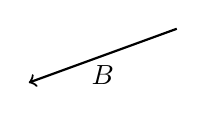
\begin{tikzpicture}
                \draw[thick,->] (0,0) -- (200:2cm);
                \node[thick,anchor=north] at (200:1cm) {$B$};
            \end{tikzpicture}
        }
    \end{choices}
    \end{multicols}
\end{question}
}

\element{nysed}{
\begin{question}{June2006-Q04}
    A golf ball is propelled with an initial velocity of
        \SI{60}{\meter\per\second} at \ang{37} above the horizontal.
    The horizontal component of the golf ball's initial velocity is:
    \begin{multicols}{2}
    \begin{choices}
      \correctchoice{\SI{48}{\meter\per\second}}
        \wrongchoice{\SI{40}{\meter\per\second}}
        \wrongchoice{\SI{30}{\meter\per\second}}
        \wrongchoice{\SI{36}{\meter\per\second}}
    \end{choices}
    \end{multicols}
\end{question}
}

\element{nysed}{
\begin{question}{June2006-Q06}
    A \SI{3}{\newton} force and a \SI{4}{\newton} force are acting concurrently on a point.
    Which force could not produce equilibrium with these two forces?
    \begin{multicols}{2}
    \begin{choices}
        \wrongchoice{\SI{1}{\newton}}
        \wrongchoice{\SI{7}{\newton}}
      \correctchoice{\SI{9}{\newton}}
        \wrongchoice{\SI{4}{\newton}}
    \end{choices}
    \end{multicols}
\end{question}
}


%% Section Jan2006
%%--------------------
\element{nysed}{
\begin{question}{Jan2006-Q04}
    A projectile is fired with an initial velocity of
        \SI{120}{\meter\per\second}
        at an angle, $\theta$, above the horizontal.
    If the projectile's initial horizontal speed is
        \SI{55}{\meter\per\second}, then angle $\theta$
        measures approximately:
    \begin{multicols}{4}
    \begin{choices}
      \correctchoice{\ang{63}}
        \wrongchoice{\ang{75}}
        \wrongchoice{\ang{27}}
        \wrongchoice{\ang{13}}
    \end{choices}
    \end{multicols}
\end{question}
}

\element{nysed}{
\begin{question}{Jan2006-Q03}
    Which is a scalar quantity?
    \begin{multicols}{2}
    \begin{choices}
      \correctchoice{speed}
        \wrongchoice{acceleration}
        \wrongchoice{displacement}
        \wrongchoice{momentum}
    \end{choices}
    \end{multicols}
\end{question}
}

\element{nysed}{
\begin{question}{Jan2006-Q12}
    A student on her way to school walks four blocks east,
        three block north, and another four blocks east,
        as shown in the diagram.
    \begin{center}
        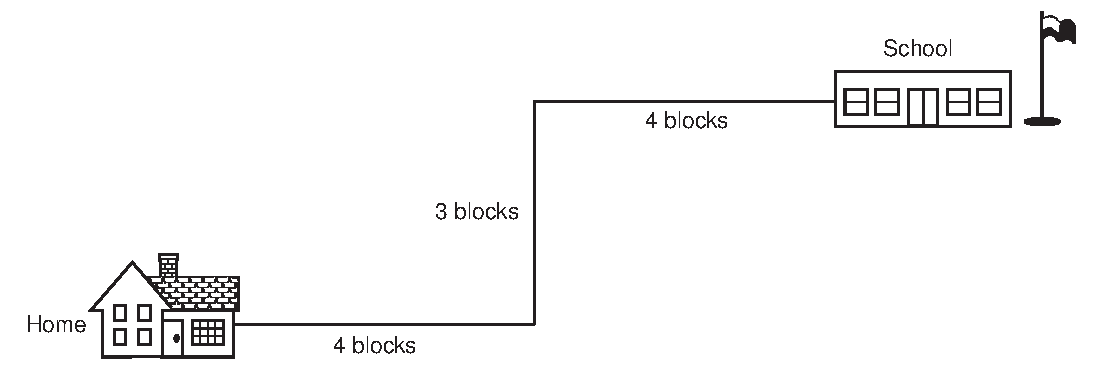
\includegraphics[keepaspectratio,width=\linewidth]{Jan2006-Q12}
    \end{center}
    Compared to the distance she walks,
        the magnitude of her displacement home to school is:
    \begin{multicols}{3}
    \begin{choices}
      \correctchoice{less}
        \wrongchoice{more}
        \wrongchoice{the same}
    \end{choices}
    \end{multicols}
\end{question}
}

\element{nysed}{
\begin{question}{Jan2006-Q46}
    Two \SI{30}{\newton} forces act concurrently on an object.
    In which diagram would the forces produce a
        resultant with a magnitude of \SI{30}{\newton}?
    \begin{multicols}{2}
    \begin{choices}
        \AMCboxDimensions{down=-1.0em}
        \correctchoice{
            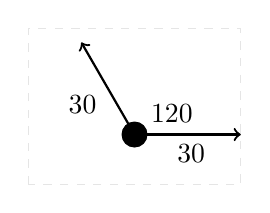
\begin{tikzpicture}[scale=0.9]
                \draw[dashed,white!90!black] (-1.5cm,-2em) rectangle (1.5cm,1.5cm);
                \draw[fill] (0,0) circle [radius=0.5em];
                \node[anchor=south west] at (15:0.1cm) {\ang{120}};
                \draw[thick,->] (0,0) -- (0:1.5cm);
                \node[anchor=north] at (0:0.8cm) {\SI{30}{\newton}};
                \draw[thick,->] (0,0) -- (120:1.5cm);
                \node[anchor=north east] at (120:0.8cm) {\SI{30}{\newton}};
            \end{tikzpicture}
        }
        \wrongchoice{
            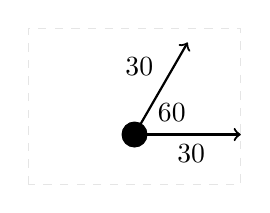
\begin{tikzpicture}[scale=0.9]
                \draw[dashed,white!90!black] (-1.5cm,-2em) rectangle (1.5cm,1.5cm);
                \draw[fill] (0,0) circle [radius=0.5em];
                \node[anchor=south west] at (15:0.2cm) {\ang{60}};
                \draw[thick,->] (0,0) -- (0:1.5cm);
                \node[anchor=north] at (0:0.8cm) {\SI{30}{\newton}};
                \draw[thick,->] (0,0) -- (60:1.5cm);
                \node[anchor=south east] at (60:0.8cm) {\SI{30}{\newton}};
            \end{tikzpicture}
        }
        \wrongchoice{
            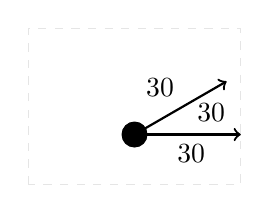
\begin{tikzpicture}[scale=0.9]
                \draw[dashed,white!90!black] (-1.5cm,-2em) rectangle (1.5cm,1.5cm);
                \draw[fill] (0,0) circle [radius=0.5em];
                \node[anchor=south west] at (4:0.75cm) {\ang{30}};
                \draw[thick,->] (0,0) -- (0:1.5cm);
                \node[anchor=north] at (0:0.8cm) {\SI{30}{\newton}};
                \draw[thick,->] (0,0) -- (30:1.5cm);
                \node[anchor=south east] at (30:0.8cm) {\SI{30}{\newton}};
            \end{tikzpicture}
        }
        \wrongchoice{
            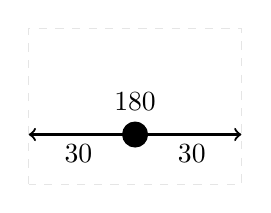
\begin{tikzpicture}[scale=0.9]
                \draw[dashed,white!90!black] (-1.5cm,-2em) rectangle (1.5cm,1.5cm);
                \draw[fill] (0,0) circle [radius=0.5em];
                \node[anchor=south] at (90:0.2cm) {\ang{180}};
                \draw[thick,->] (0,0) -- (0:1.5cm);
                \node[anchor=north] at (0:0.8cm) {\SI{30}{\newton}};
                \draw[thick,->] (0,0) -- (180:1.5cm);
                \node[anchor=north] at (180:0.8cm) {\SI{30}{\newton}};
            \end{tikzpicture}
        }
    \end{choices}
    \end{multicols}
\end{question}
}


%% Section June2005
%%--------------------
\element{nysed}{
\begin{question}{June2005-Q03}
    A \SI{5.0}{\newton} force and a \SI{7.0}{\newton} force act concurrently on a point.
    As the angle between the forces is increased from \ang{0} to \ang{180},
        the magnitude of the resultant of the two forces changes from:
    \begin{multicols}{2}
    \begin{choices}
      \correctchoice{\SI{12.0}{\newton} to \SI{2.0}{\newton}}
        \wrongchoice{\SI{0.0}{\newton} to \SI{12.0}{\newton}}
        \wrongchoice{\SI{2.0}{\newton} to \SI{12.0}{\newton}}
        \wrongchoice{\SI{12.0}{\newton} to \SI{0.0}{\newton}}
    \end{choices}
    \end{multicols}
\end{question}
}

\element{nysed}{
\begin{question}{June2005-Q04}
    A \SI{5.0}{\newton} force could have perpendicular components of:
    \begin{multicols}{2}
    \begin{choices}
      \correctchoice{\SI{3.0}{\newton} and \SI{4.0}{\newton}}
        \wrongchoice{\SI{1.0}{\newton} and \SI{4.0}{\newton}}
        \wrongchoice{\SI{2.0}{\newton} and \SI{3.0}{\newton}}
        \wrongchoice{\SI{5.0}{\newton} and \SI{5.0}{\newton}}
    \end{choices}
    \end{multicols}
\end{question}
}


%% Section Jan2005
%%--------------------
\element{nysed}{
\begin{question}{Jan2005-Q03}
    A golf ball is hit with an initial velocity of \SI{15}{\meter\per\second} at an angle of \ang{35} above the horizontal.
    What is the vertical component of the gold ball's initial velocity?
    \begin{multicols}{2}
    \begin{choices}
      \correctchoice{\SI{8.6}{\meter\per\second}}
        \wrongchoice{\SI{9.8}{\meter\per\second}}
        \wrongchoice{\SI{12}{\meter\per\second}}
        \wrongchoice{\SI{15}{\meter\per\second}}
    \end{choices}
    \end{multicols}
\end{question}
}

\element{nysed}{
\begin{question}{Jan2005-Q37}
    The vector below represents two forces, $F_1$ and $F_2$, simultaneously acting on an object.
    \begin{center}
    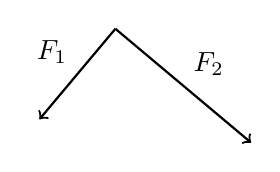
\begin{tikzpicture}[scale=0.75]
        \draw[thick,->] (0,0) -- (230:2cm)
            node[pos=0.5,anchor=south east] {$F_1$};
        \draw[thick,->] (0,0) -- (320:3cm)
            node[pos=0.5,anchor=south west] {$F_2$};
    \end{tikzpicture}
    \end{center}
    Which vector best represents the resultant of the two forces?
    \begin{multicols}{2}
    \begin{choices}
        \AMCboxDimensions{down=-1.5em}
        \correctchoice{
            \begin{tikzpicture}[scale=0.75]
                \draw[dashed,white!90!black] (-1.00,-3.5) rectangle (2.50,0);
                \draw[thick,->] (0,0) -- (286:3.6cm)
                    node[pos=0.5,anchor=east] {$R$};
            \end{tikzpicture}
        }
        \wrongchoice{
            \begin{tikzpicture}[scale=0.75]
                \draw[dashed,white!90!black] (+1.00,+3.5) rectangle (-2.50,-0);
                \draw[thick,->] (0,0) -- (106:3.6cm)
                    node[pos=0.5,anchor=east] {$R$};
            \end{tikzpicture}
        }
        \wrongchoice{
            \begin{tikzpicture}[scale=0.75]
                \draw[dashed,white!90!black] (+0.25,+2) rectangle (-3.75,-1.5);
                \draw[thick,->] (0,0) -- (176:3.6cm)
                    node[pos=0.5,anchor=south west] {$R$};
            \end{tikzpicture}
        }
        \wrongchoice{
            \begin{tikzpicture}[scale=0.75]
                \draw[dashed,white!90!black] (-0.25,-2) rectangle (3.75,1.5);
                \draw[thick,->] (0,0) -- (356:3.6cm)
                    node[pos=0.5,anchor=south west] {$R$};
            \end{tikzpicture}
        }
    \end{choices}
    \end{multicols}
\end{question}
}


%% Section June2004
%%--------------------
\element{nysed}{
\begin{question}{June2004-Q01}
    Velocity is to speed as displacement is to:
    \begin{multicols}{2}
    \begin{choices}
      \correctchoice{distance}
        \wrongchoice{acceleration}
        \wrongchoice{time}
        \wrongchoice{momentum}
    \end{choices}
    \end{multicols}
\end{question}
}

\element{nysed}{
\begin{question}{June2004-Q02}
    The diagram below shows a resultant vector, $R$.
    \begin{center}
    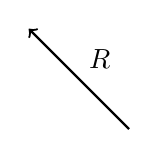
\begin{tikzpicture}[scale=0.9]
        \draw[thick,->] (0,0) -- (135:2cm)
            node[pos=0.5,anchor=south west] {$R$};
    \end{tikzpicture}
    \end{center}
    Which diagram best represents a pair of component vectors, $A$ and $B$,
        that would combine to form resultant vector $R$?
    \begin{multicols}{2}
    \begin{choices}
        \AMCboxDimensions{down=-0.5cm}
        \correctchoice{
            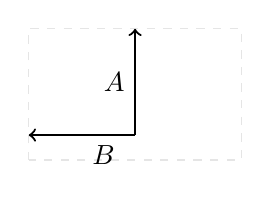
\begin{tikzpicture}[scale=0.9]
                \draw[dashed,white!90!black] (-1.5cm,-1em) rectangle (1.5cm,1.5cm);
                \draw[thick,->] (0,0) -- (90:1.5cm)
                    node[pos=0.5,anchor=east] {$A$};
                \draw[thick,->] (0,0) -- (180:1.5cm)
                    node[pos=0.5,anchor=north west] {$B$};
            \end{tikzpicture}
        }
        \wrongchoice{
            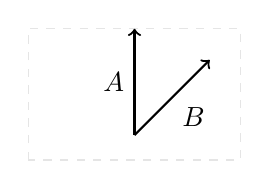
\begin{tikzpicture}[scale=0.9]
                \draw[dashed,white!90!black] (-1.5cm,-1em) rectangle (1.5cm,1.5cm);
                \draw[thick,->] (0,0) -- (90:1.5cm)
                    node[pos=0.5,anchor=east] {$A$};
                \draw[thick,->] (0,0) -- (45:1.5cm)
                    node[pos=0.5,anchor=north west] {$B$};
            \end{tikzpicture}
        }
        \wrongchoice{
            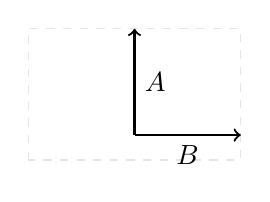
\begin{tikzpicture}[scale=0.9]
                \draw[dashed,white!90!black] (-1.5cm,-1em) rectangle (1.5cm,1.5cm);
                \draw[thick,->] (0,0) -- (90:1.5cm)
                    node[pos=0.5,anchor=west] {$A$};
                \draw[thick,->] (0,0) -- (0:1.5cm)
                    node[pos=0.5,anchor=north] {$B$};
            \end{tikzpicture}
        }
        \wrongchoice{
            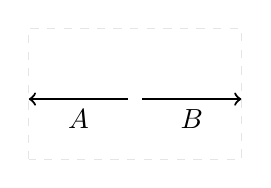
\begin{tikzpicture}[scale=0.9]
                \draw[dashed,white!90!black] (-1.5cm,-1em-0.50cm) rectangle (1.5cm,1.00cm);
                \draw[thick,->] (-0.1cm,0) -- (180:1.5cm)
                    node[pos=0.5,anchor=north] {$A$};
                \draw[thick,->] (0.1cm,0) -- (0:1.5cm)
                    node[pos=0.5,anchor=north] {$B$};
            \end{tikzpicture}
        }
    \end{choices}
    \end{multicols}
\end{question}
}


%% Section Jan2004
%%--------------------
\element{nysed}{
\begin{question}{Jan2004-Q01}
    A girl leaves a history classroom and walks \SI{10}{\meter} north to a drinking fountain.
    Then she turns and walks \SI{30}{\meter} south to an art classroom.
    What is the girl's total displacement from the history classroom to the art classroom?
    \begin{multicols}{2}
    \begin{choices}
      \correctchoice{\SI{20.}{\meter} south}
        \wrongchoice{\SI{20.}{\meter} north}
        \wrongchoice{\SI{40.}{\meter} south}
        \wrongchoice{\SI{40.}{\meter} north}
    \end{choices}
    \end{multicols}
\end{question}
}

\element{nysed}{
\begin{question}{Jan2004-Q02}
    One car travels \SI{40}{\meter} due east in \SI{5.0}{\second},
        and a second car travels \SI{64}{\meter} due west in \SI{8.0}{\second}.
    During their periods of travel, the cars definitely had the same
    \begin{choices}
      \correctchoice{average speed}
        \wrongchoice{average velocity}
        \wrongchoice{total displacement}
        \wrongchoice{change in momentum}
    \end{choices}
\end{question}
}

\element{nysed}{
\begin{question}{Jan2004-Q39}
    The diagram below represents a \SI{5.0}{\newton} force and a \SI{12}{\newton} force acting on point $P$.
    \begin{center}
    \begin{tikzpicture}
        \node[anchor=north east] at (0:0) {$P$};
        \draw[fill] (0,0) circle [radius=2pt];
        \draw[thick,->] (0,0) -- (90:2cm);
        \node[anchor=south,rotate=90] at (90:1cm) {\SI{5}{\newton}};
        \draw[thick,->] (0,0) -- (0:4.8cm);
        \node[anchor=north] at (0:2.4cm) {\SI{12}{\newton}};
    \end{tikzpicture}
    \end{center}
    The resultant of the two forces has magnitude of:
    \begin{multicols}{2}
    \begin{choices}
      \correctchoice{\SI{13}{\newton}}
        \wrongchoice{\SI{12}{\newton}}
        \wrongchoice{\SI{5.0}{\newton}}
        \wrongchoice{\SI{7.0}{\newton}}
    \end{choices}
    \end{multicols}
\end{question}
}


%% Section June2003
%%--------------------
\element{nysed}{
\begin{question}{June2003-Q02}
    A vector makes an angle $\theta$ with the horizontal.
    The horizontal and vertical components of the vector will be equal in magnitude if angle $\theta$ is:
    \begin{multicols}{4}
    \begin{choices}
      \correctchoice{\ang{45}}
        \wrongchoice{\ang{30}}
        \wrongchoice{\ang{60}}
        \wrongchoice{\ang{90}}
    \end{choices}
    \end{multicols}
\end{question}
}

\element{nysed}{
\begin{question}{June2003-Q36}
    Force $A$ and $B$ have a resultant $R$. 
    Force $A$ and resultant $R$ are represented in the diagram below.
    \begin{center}
    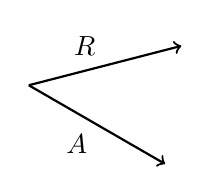
\begin{tikzpicture}
        \draw[thick,->] (0,0) -- (14.47:2cm);
        \node[anchor=south east] at (14.47:1cm) {$R$};
        \draw[thick,->] (0,0) -- (-30:2cm);
        \node[anchor=north east] at (-30:1cm) {$A$};
    \end{tikzpicture}
    \end{center}
    Which vector best represents force $B$?
    \begin{multicols}{2}
    \begin{choices}
        \AMCboxDimensions{down=-0.5cm}
        \correctchoice{
            \begin{tikzpicture}
                \draw[draw=white] (-0.75,0) rectangle (0.75,1);
                \draw[thick,->] (0,0) -- (90:1cm)
                    node[pos=0.5,anchor=east] {$B$};
            \end{tikzpicture}
        }
        \wrongchoice{
            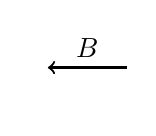
\begin{tikzpicture}
                \draw[draw=white] (-0.25,-0.5) rectangle (-1.25,0.5);
                \draw[thick,->] (0,0) -- (180:1cm)
                    node[pos=0.5,anchor=south] {$B$};
            \end{tikzpicture}
        }
        \wrongchoice{
            \begin{tikzpicture}
                \draw[draw=white] (-0.75,0) rectangle (0.75,-1);
                \draw[thick,->] (0,0) -- (270:1cm)
                    node[pos=0.5,anchor=east] {$B$};
            \end{tikzpicture}
        }
        \wrongchoice{
            \begin{tikzpicture}
                \draw[draw=white] (-0.25,-0.5) rectangle (1.25,0.5);
                \draw[thick,->] (0,0) -- (0:1cm)
                    node[pos=0.5,anchor=south] {$B$};
            \end{tikzpicture}
        }
    \end{choices}
    \end{multicols}
\end{question}
}


%% Section Jan2003
%%--------------------
\element{nysed}{
\begin{question}{Jan2003-Q02}
    A car travels \SI{90}{\meter} due north in \SI{15}{\second}.
    Then the car turns around and travels \SI{40}{\meter} due south in \SI{5.0}{\second}.
    What is the magnitude of the average velocity of the car during this \SI{20}{\second} interval?
    \begin{multicols}{2}
    \begin{choices}
      \correctchoice{\SI{2.5}{\meter\per\second}}
        \wrongchoice{\SI{5.0}{\meter\per\second}}
        \wrongchoice{\SI{6.5}{\meter\per\second}}
        \wrongchoice{\SI{7.0}{\meter\per\second}}
    \end{choices}
    \end{multicols}
\end{question}
}

\element{nysed}{
\begin{question}{Jan2003-Q36}
    Which pair of forces acting concurrently on an object will produce the resultant of greatest magnitude?
    \begin{multicols}{2}
    \begin{choices}
        \AMCboxDimensions{down=-0.5em}
        \correctchoice{
            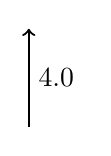
\begin{tikzpicture}
                \draw[thick,->] (0,0) -- (90:1.25cm);
                \node[anchor=west] at (90:0.625cm) {\SI{4.0}{\newton}};
            \end{tikzpicture}
            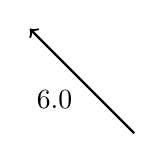
\begin{tikzpicture}
                \draw[thick,->] (0,0) -- (135:1.875cm);
                \node[anchor=north east] at (135:0.9375cm) {\SI{6.0}{\newton}};
            \end{tikzpicture}
        }
        \wrongchoice{
            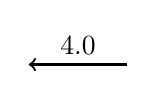
\begin{tikzpicture}
                \draw[thick,->] (0,0) -- (180:1.25cm);
                \node[anchor=south] at (180:0.625cm) {\SI{4.0}{\newton}};
            \end{tikzpicture}
            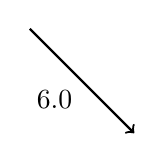
\begin{tikzpicture}
                \draw[thick,->] (0,0) -- (-45:1.875cm);
                \node[anchor=north east] at (-45:0.9375cm) {\SI{6.0}{\newton}};
            \end{tikzpicture}
        }
        \wrongchoice{
            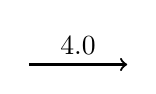
\begin{tikzpicture}
                \draw[thick,->] (0,0) -- (0:1.25cm);
                \node[anchor=south] at (0:0.625cm) {\SI{4.0}{\newton}};
            \end{tikzpicture}
            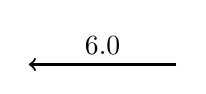
\begin{tikzpicture}
                \draw[thick,->] (0,0) -- (180:1.875cm);
                \node[anchor=south] at (180:0.9375cm) {\SI{6.0}{\newton}};
            \end{tikzpicture}
        }
        \wrongchoice{
            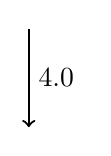
\begin{tikzpicture}
                \draw[thick,->] (0,0) -- (270:1.25cm);
                \node[anchor=west] at (270:0.625cm) {\SI{4.0}{\newton}};
            \end{tikzpicture}
            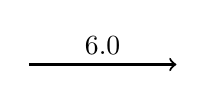
\begin{tikzpicture}
                \draw[thick,->] (0,0) -- (0:1.875cm);
                \node[anchor=south] at (0:0.9375cm) {\SI{6.0}{\newton}};
            \end{tikzpicture}
        }
    \end{choices}
    \end{multicols}
\end{question}
}


%% Section Aug2002
%%--------------------
\element{nysed}{
\begin{question}{Aug2002-Q07}
    Which term represents a scalar quantity?
    \begin{multicols}{2}
    \begin{choices}
      \correctchoice{distance}
        \wrongchoice{displacement}
        \wrongchoice{force}
        \wrongchoice{weight}
    \end{choices}
    \end{multicols}
\end{question}
}

\element{nysed}{
\begin{question}{Aug2002-Q40}
    Which vector diagram represents the greatest magnitude of displacement for an object?
    \begin{multicols}{2}
    \begin{choices}
        \AMCboxDimensions{down=-1.3cm}
        \wrongchoice{
            \begin{tikzpicture}[scale=2]
                \draw[dashed,white!90!black] (-1.3,-0.4) rectangle (0.3,1.3);
                \draw[very thick,->] (0,0) -- (0,1) node[pos=0.5,anchor=south,rotate=-90] {\SI{1}{\meter}};
            \end{tikzpicture}
        }
        \correctchoice{
            \begin{tikzpicture}[scale=2]
                \draw[dashed,white!90!black] (-1.3,-0.4) rectangle (0.3,1.3);
                \draw[very thick,->] (0,0) -- (0,1) node[pos=0.5,anchor=south,rotate=-90] {\SI{1}{\meter}};
                \draw[very thick,->] (0,1) -- (-1,1) node[pos=0.5,anchor=south] {\SI{1}{\meter}};
            \end{tikzpicture}
        }
        \wrongchoice{
            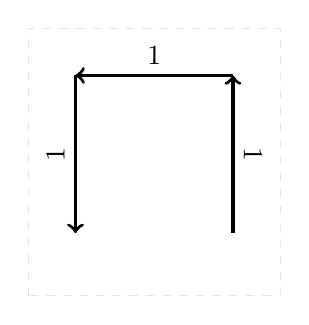
\begin{tikzpicture}[scale=2]
                \draw[dashed,white!90!black] (-1.3,-0.4) rectangle (0.3,1.3);
                \draw[very thick,->] (0,0) -- (0,1) node[pos=0.5,anchor=south,rotate=-90] {\SI{1}{\meter}};
                \draw[very thick,->] (0,1) -- (-1,1) node[pos=0.5,anchor=south] {\SI{1}{\meter}};
                \draw[very thick,->] (-1,1) -- (-1,0) node[pos=0.5,rotate=90,anchor=south] {\SI{1}{\meter}};
            \end{tikzpicture}
        }
        \wrongchoice{
            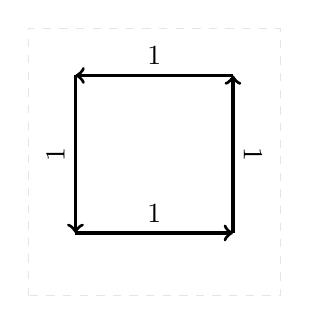
\begin{tikzpicture}[scale=2]
                \draw[dashed,white!90!black] (-1.3,-0.4) rectangle (0.3,1.3);
                \draw[very thick,->] (0,0) -- (0,1) node[pos=0.5,anchor=south,rotate=-90] {\SI{1}{\meter}};
                \draw[very thick,->] (0,1) -- (-1,1) node[pos=0.5,anchor=south] {\SI{1}{\meter}};
                \draw[very thick,->] (-1,1) -- (-1,0) node[pos=0.5,rotate=90,anchor=south] {\SI{1}{\meter}};
                \draw[very thick,->] (-1,0) -- (0,0) node[pos=0.5,anchor=south] {\SI{1}{\meter}};
            \end{tikzpicture}
        }
    \end{choices}
    \end{multicols}
\end{question}
}


%% Section June2002
%%--------------------
\element{nysed}{
\begin{question}{June2002-Q44}
    A force vector was resolved into two perpendicular components,
        $F_1$ and $F_2$, as shown in the diagram below.
    \begin{center}
    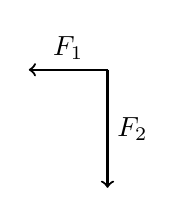
\begin{tikzpicture}
        \draw[thick,->] (0,0) -- (180:1.00cm);
        \node[anchor=south] at (180:0.5cm) {$F_1$};
        \draw[thick,->] (0,0) -- (270:1.50cm);
        \node[anchor=west] at (270:0.75cm) {$F_2$};
    \end{tikzpicture}
    \end{center}
    Which vector best represents the original force?
    \begin{multicols}{2}
    \begin{choices}
        \AMCboxDimensions{down=-1.0cm}
        \correctchoice{
            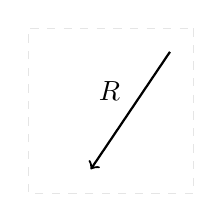
\begin{tikzpicture}
                \draw[dashed,white!90!black] (0.3,0.3) rectangle (-1.8,-1.8);
                \draw[thick,->] (0,0) -- (236:1.8cm)
                    node[pos=0.5,anchor=south east] {$R$};
            \end{tikzpicture}
        }
        \wrongchoice{
            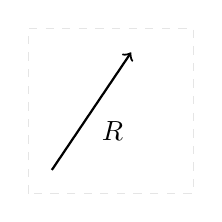
\begin{tikzpicture}
                \draw[dashed,white!90!black] (-0.3,-0.3) rectangle (1.8,1.8);
                \draw[thick,->] (0,0) -- (56:1.8cm)
                    node[pos=0.5,anchor=north west] {$R$};
            \end{tikzpicture}
        }
        \wrongchoice{
            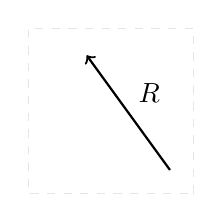
\begin{tikzpicture}
                \draw[dashed,white!90!black] (0.3,-0.3) rectangle (-1.8,1.8);
                \draw[thick,->] (0,0) -- (126:1.8cm)
                    node[pos=0.5,anchor=south west] {$R$};
            \end{tikzpicture}
        }
        \wrongchoice{
            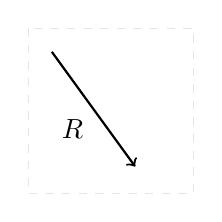
\begin{tikzpicture}
                \draw[dashed,white!90!black] (-0.3,0.3) rectangle (1.8,-1.8);
                \draw[thick,->] (0,0) -- (306:1.8cm)
                    node[pos=0.5,anchor=north east] {$R$};
            \end{tikzpicture}
        }
    \end{choices}
    \end{multicols}
\end{question}
}


%% Section Jan2002
%%--------------------
\element{nysed}{
\begin{question}{Jan2002-Q01}
    What is the total displacement of a student who walks \num{3} blocks east,
        \num{2} blocks north, \num{1} block west,
        and then \num{2} blocks south?
    \begin{multicols}{2}
    \begin{choices}
        \wrongchoice{\num{0}}
      \correctchoice{\num{2} blocks east}
        \wrongchoice{\num{2} blocks west}
        \wrongchoice{\num{8} blocks}
    \end{choices}
    \end{multicols}
\end{question}
}

\element{nysed}{
\begin{question}{Jan2002-Q08}
    Two concurrent forces have a maximum resultant of \SI{45}{\newton} and a minimum resultant of \SI{5}{\newton}.
    What is the magnitude of each of these forces?
    \begin{multicols}{2}
    \begin{choices}
        \wrongchoice{\SI{0}{\newton} and \SI{45}{\newton}}
        \wrongchoice{\SI{5}{\newton} and \SI{9}{\newton}}
      \correctchoice{\SI{20}{\newton} and \SI{25}{\newton}}
        \wrongchoice{\SI{0}{\newton} and \SI{50}{\newton}}
    \end{choices}
    \end{multicols}
\end{question}
}


%% Section June2001
%%-------------------
\element{nysed}{
\begin{question}{June2001-Q01}
    Which terms both represents scalar quantities?
    \begin{choices}
        \wrongchoice{displacement and velocity}
      \correctchoice{distance and speed}
        \wrongchoice{displacement and speed}
        \wrongchoice{distance and velocity}
    \end{choices}
\end{question}
}

\element{nysed}{
\begin{question}{June2001-Q06}
    Two students push on a sled.
    One pushes with a force of \SI{30}{\newton} east and the other exerts a force of \SI{40}{\newton} south,
        as shown in the topview diagram below.
    \begin{center}
    \begin{tikzpicture}
        \draw (0,0) rectangle (1.5cm,1.0cm);
        \node[anchor=south,yshift=-3pt] at (0.75cm,0.50cm) {Top of};
        \node[anchor=north,yshift=3pt] at (0.75cm,0.50cm) {sled};
        \draw[thick,->] (0.75cm,0) -- (0.75cm,-1.2cm);
        \node[anchor=south west] at (0.75cm,-1.2cm) {\SI{40}{\newton} south};
        \draw[thick,->] (1.5cm,0.50cm) -- (2.4cm,0.50cm);
        \node[anchor=west] at (2.4cm,0.50cm) {\SI{30}{\newton} east};
    \end{tikzpicture}
    \end{center}
    Which vector best represents the resultant of these two forces?
    %% NOTE: I think the wrong direction should be 180 from correct
    \begin{multicols}{2}
    \begin{choices}
        \AMCboxDimensions{down=-0.5cm}
        \correctchoice{
            \begin{tikzpicture}
                \draw[draw=white] (0,0.3) rectangle (1.5,-1.2);
                \draw[thick,->] (0,0) -- (-45:1.5cm);
                \node[thick,anchor=south west] at (-45:0.75cm) {\SI{50}{\newton}};
            \end{tikzpicture}
        }
        \wrongchoice{
            \begin{tikzpicture}
                \draw[draw=white] (0,-0.3) rectangle (1.5,1.2);
                \draw[thick,->] (0,0) -- (45:1.5cm);
                \node[thick,anchor=north west] at (45:0.75cm) {\SI{50}{\newton}};
            \end{tikzpicture}
        }
        \wrongchoice{
            \begin{tikzpicture}
                \draw[draw=white] (0,0) rectangle (1.5,-1.5);
                \draw[thick,->] (0,0) -- (-45:2.1cm);
                \node[thick,anchor=south west] at (-45:1.05cm) {\SI{70}{\newton}};
            \end{tikzpicture}
        }
        \wrongchoice{
            \begin{tikzpicture}
                \draw[draw=white] (0,0) rectangle (1.5,1.5);
                \draw[thick,->] (0,0) -- (45:2.1cm);
                \node[thick,anchor=north west] at (45:1.05cm) {\SI{70}{\newton}};
            \end{tikzpicture}
        }
    \end{choices}
    \end{multicols}
\end{question}
}

\element{nysed}{
\begin{question}{June2001-Q56}
    A football player kicks a ball with an initial velocity of \SI{25}{\meter\per\second} at an angle of \ang{53} above the horizontal.
    The vertical component of the initial velocity of the ball is:
    \begin{multicols}{2}
    \begin{choices}
        \wrongchoice{\SI{25}{\meter\per\second}}
      \correctchoice{\SI{20}{\meter\per\second}}
        \wrongchoice{\SI{15}{\meter\per\second}}
        \wrongchoice{\SI{10}{\meter\per\second}}
    \end{choices}
    \end{multicols}
\end{question}
}


%% Section Jan2001
%%--------------------
\element{nysed}{
\begin{question}{Jan2001-Q03}
    The diagram below shows a block on a horizontal frictionless surface.
    A \SI{100}{\newton} force acts on the block at an angle of \ang{30} above the horizontal.
    \begin{center}
    \begin{tikzpicture}
        %% Unknown Force
        \draw[thick,->] (-1,0.5) -- (-3,0.5)
            node[pos=0.66,anchor=south] {$F$};
        %% Known Force
        \draw[dashed,thick,->] (1,0.5) -- (2.667,0.5)
            node[pos=0.5,anchor=south west] {\ang{30}};
        \draw[thick,->] (1,0.5) -- ++(30:3)
            node[pos=0.5,anchor=south,rotate=30] {\SI{100}{\newton}};
        %% Block
        \draw[thick] (-1,0) rectangle (1,1);
        \node[anchor=center] at (0,0.5) {Block};
        %% Floor
        \draw[thick] (-3.0,0) -- (3.0,0);
        \foreach \x in {-30,-29,...,30}
            \draw[thin] (\x mm,0cm) -- ++ (220:0.15cm);
        \node[anchor=north] at (0,-0.15) {Frictionless surface};
    \end{tikzpicture}
    \end{center}
    What is the magnitude of force $F$ if it establishes equilibrium?
    \begin{multicols}{2}
    \begin{choices}
        \wrongchoice{\SI{50.0}{\newton}}
        \wrongchoice{\SI{100}{\newton}}
      \correctchoice{\SI{86.6}{\newton}}
        \wrongchoice{\SI{187}{\newton}}
    \end{choices}
    \end{multicols}
\end{question}
}

\element{nysed}{
\begin{question}{Jan2001-Q05}
    A \SI{5}{\newton} force directed east and a \SI{5}{\newton} force directed north act concurrently on a point.
    The resultant of the two forces is:
    \begin{multicols}{2}
    \begin{choices}
        \wrongchoice{\SI{5.0}{\newton} northeast}
        \wrongchoice{\SI{10}{\newton} southwest}
      \correctchoice{\SI{7}{\newton} northeast}
        \wrongchoice{\SI{7}{\newton} southwest}
    \end{choices}
    \end{multicols}
\end{question}
}

\element{nysed}{
\begin{question}{Jan2001-Q06}
    Into how many possible components can a single force be resolved?
    \begin{choices}
        \wrongchoice{an unlimited number}
        \wrongchoice{two components}
      \correctchoice{three components}
        \wrongchoice{four components at right angles to each other}
    \end{choices}
\end{question}
}

\element{nysed}{
\begin{question}{Jan2001-Q63}
    A projectile is launched with an initial velocity of \SI{200}{\meter\per\second} at \ang{30} above the horizontal.
    What is the magnitude of the vertical component of the projectile's initial velocity?
    \begin{multicols}{2}
    \begin{choices}
        \wrongchoice{$\SI{200}{\meter\per\second} \times \cos{\ang{30}}$}
      \correctchoice{$\SI{200}{\meter\per\second} \times \sin{\ang{30}}$}
        \wrongchoice{$\dfrac{\SI{200}{\meter\per\second}}{\sin{\ang{30}}}$}
        \wrongchoice{$\dfrac{\SI{200}{\meter\per\second}}{\cos{\ang{30}}}$}
    \end{choices}
    \end{multicols}
\end{question}
}


%% Section June2000
%%--------------------
\element{nysed}{
\begin{question}{June2000-Q01}
    The map below shows the route traveled by a school bus.
    \begin{center}
        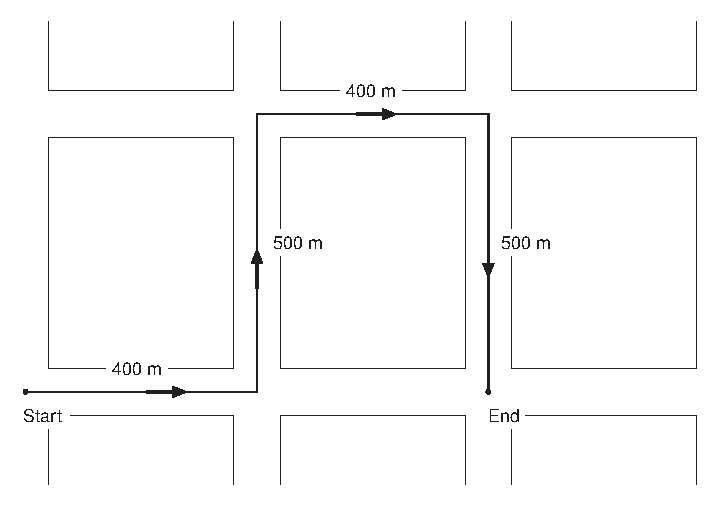
\includegraphics[keepaspectratio,width=\linewidth]{June2000-Q01}
    \end{center}
    What is the magnitude of the total displacement of the school bus from the start to the end of its trip?
    \begin{multicols}{2}
    \begin{choices}
        \wrongchoice{\SI{400}{\meter}}
        \wrongchoice{\SI{500}{\meter}}
      \correctchoice{\SI{800}{\meter}}
        \wrongchoice{\SI{1800}{\meter}}
    \end{choices}
    \end{multicols}
\end{question}
}

\element{nysed}{
\begin{question}{June2000-Q05}
    In the diagram below, a force, $F$, is applied to the handle of a lawnmower inclined at angle $\theta$ to the ground.
    \begin{center}
        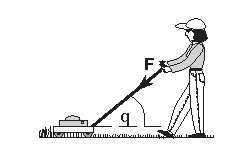
\includegraphics[keepaspectratio,scale=1.0]{June2000-Q05}
    \end{center}
    The magnitude of the horizontal component of force $F$ depends on:
    \begin{choices}
        \wrongchoice{the magnitude of the force $F$, only}
        \wrongchoice{the measure of angle $\theta$, only}
      \correctchoice{both the magnitude of force $F$ and the measure of angle $\theta$.}
        \wrongchoice{neither the magnitude of force $F$ nor the measure of angle $\theta$.}
    \end{choices}
\end{question}
}


\element{nysed}{
\begin{question}{June2000-Q06}
    Equilibrium exists in a system where three forces are acting concurrently on an object.
    If the system includes a \SI{5.0}{\newton} force due north and a \SI{2.0}{\newton} force due south, the third force must be:
    \begin{multicols}{2}
    \begin{choices}
        \wrongchoice{\SI{7.0}{\newton} south}
        \wrongchoice{\SI{7.0}{\newton} north}
      \correctchoice{\SI{3.0}{\newton} south}
        \wrongchoice{\SI{3.0}{\newton} north}
    \end{choices}
    \end{multicols}
\end{question}
}

\element{nysed}{
\begin{question}{June2000-Q09}
    Which term represents a vector quantity and its respective unit?
    \begin{multicols}{2}
    \begin{choices}
        \wrongchoice{weight (\si{\kilo\gram})}
        \wrongchoice{mass (\si{\kilo\gram})}
      \correctchoice{force (\si{\newton})}
        \wrongchoice{momentum (\si{\newton})}
    \end{choices}
    \end{multicols}
\end{question}
}

\element{nysed}{
\begin{question}{June2000-Q10}
    The vector below represents the resultant of two forces acting concurrently on an object at point $P$.
    \begin{center}
    \begin{tikzpicture}
        \draw[fill] (0,0) circle [radius=2pt];
        \node[anchor=west] at (0,0) {$P$};
        \draw[thick,->] (0,0) -- (150:3.00cm);
        \node[anchor=south,rotate=-30] at (150:1.5cm) {Resultant};
    \end{tikzpicture}
    \end{center}
    Which pair of vectors best represents two concurrent forces that combine to produce this resultant force vector?
    \begin{multicols}{2}
    \begin{choices}
        \AMCboxDimensions{down=-1.0cm}
        \correctchoice{
            \begin{tikzpicture}[scale=0.75]
                \draw[draw=white] (-2cm,-1cm) rectangle (2cm,1cm);
                \draw[fill] (0,0) circle [radius=2pt];
                \node[anchor=north] at (0,0) {$P$};
                \draw[thick,->] (0,0) -- (0:1.5cm);
                \draw[thick,->] (0,0) -- (120:1.5cm);
            \end{tikzpicture}
        }
        \wrongchoice{
            \begin{tikzpicture}[scale=0.75]
                \draw[draw=white] (-2cm,-1cm) rectangle (2cm,1.3cm);
                \draw[fill] (0,0) circle [radius=2pt];
                \node[anchor=east] at (0,0) {$P$};
                \draw[thick,->] (0,0) -- (0:2cm);
                \draw[thick,->] (0,0) -- (90:1cm);
            \end{tikzpicture}
        }
        \wrongchoice{
            \begin{tikzpicture}[scale=0.75]
                \draw[draw=white] (-2cm,-1cm) rectangle (2cm,1cm);
                \draw[fill] (0,0) circle [radius=2pt];
                \node[anchor=south] at (0,0) {$P$};
                \draw[thick,->] (0,0) -- (180:2cm);
                \draw[thick,->] (0,0) -- (270:1cm);
            \end{tikzpicture}
        }
        \wrongchoice{
            \begin{tikzpicture}[scale=0.75]
                \draw[draw=white] (-2cm,-1cm) rectangle (2cm,1cm);
                \draw[fill] (0,0) circle [radius=2pt];
                \node[anchor=west] at (0,0) {$P$};
                \draw[thick,->] (0,0) -- (180:1.5cm);
                \draw[thick,->] (0,0) -- (120:1.5cm);
            \end{tikzpicture}
        }
    \end{choices}
    \end{multicols}
\end{question}
}


%% Section June1999
%%--------------------
\element{nysed}{
\begin{question}{June1999-Q01}
    A shown in the diagram below,
        a painter climbs \SI{7.3}{\meter} up a vertical scaffold from $A$ to $B$ and then walks \SI{11}{\meter} from $B$ to $C$ along a level platform.
    \begin{center}
        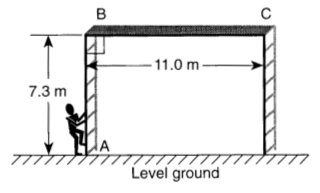
\includegraphics[keepaspectratio,scale=0.80]{June1999-Q01}
    \end{center}
    The magnitude of the painter's total displacement while moving from $A$ to $C$ is:
    \begin{multicols}{2}
    \begin{choices}
        \wrongchoice{\SI{3.7}{\meter}}
      \correctchoice{\SI{13.2}{\meter}}
        \wrongchoice{\SI{18.3}{\meter}}
        \wrongchoice{\SI{25.6}{\meter}}
    \end{choices}
    \end{multicols}
\end{question}
}

\element{nysed}{
\begin{question}{June1999-Q07}
    Which combination of three concurrent forces acting on a body could \emph{not} produce equilibrium?
    \begin{multicols}{2}
    \begin{choices}
      \correctchoice{\SI{1}{\newton},\SI{3}{\newton},\SI{5}{\newton}}
        \wrongchoice{\SI{2}{\newton},\SI{2}{\newton},\SI{2}{\newton}}
        \wrongchoice{\SI{3}{\newton},\SI{4}{\newton},\SI{5}{\newton}}
        \wrongchoice{\SI{4}{\newton},\SI{4}{\newton},\SI{5}{\newton}}
    \end{choices}
    \end{multicols}
\end{question}
}


%% Section June1998
%%--------------------
\element{nysed}{
\begin{question}{June1998-Q01}
    A car travels \SI{12}{\kilo\meter} due north and then \SI{8}{\kilo\meter} due west going from town $A$ to town $B$.
    What is the magnitude of the displacement of a helicopter that flies in a straight line from town $A$ to town $B$?
    \begin{multicols}{2}
    \begin{choices}
        \wrongchoice{\SI{20}{\kilo\meter}}
      \correctchoice{\SI{14}{\kilo\meter}}
        \wrongchoice{\SI{10}{\kilo\meter}}
        \wrongchoice{\SI{4}{\kilo\meter}}
    \end{choices}
    \end{multicols}
\end{question}
}

\element{nysed}{
\begin{question}{June1998-Q04}
    Forces $F_1$ and $F_2$ act concurrently on point $P$,
        as shown in the diagram below.
    \begin{center}
    \begin{tikzpicture}
        \draw[fill] (0,0) circle [radius=2pt];
        \node[anchor=north east] at (0,0) {$P$};

        \draw[thick,->] (0,0) -- (0:3.00cm);
        \node[anchor=north] at (0:1.50cm) {$F_2=\SI{10}{\newton}$ east};

        \draw[thick,->] (0,0) -- (90:3.00cm);
        \node[anchor=south,rotate=90] at (90:1.50cm) {$F_1=\SI{10}{\newton}$ north};
    \end{tikzpicture}
    \end{center}
    The equilibrant of $F_1$ and $F_2$ is:
    \begin{multicols}{2}
    \begin{choices}
      \correctchoice{\SI{14}{\newton} southwest}
        \wrongchoice{\SI{14}{\newton} southeast}
        \wrongchoice{\SI{20}{\newton} southwest}
        \wrongchoice{\SI{20}{\newton} southeast}
    \end{choices}
    \end{multicols}
\end{question}
}

\element{nysed}{
\begin{question}{June1998-Q61}
    An artillery shell is fired at an angle to the horizontal.
    Its initial velocity has a vertical component of \SI{150}{\meter\per\second} and a horizontal component of \SI{260}{\meter\per\second}.
    What is the magnitude of the initial velocity of the shell?
    \begin{multicols}{2}
    \begin{choices}
        \wrongchoice{\SI{9.0e4}{\meter\per\second}}
        \wrongchoice{\SI{4.1e2}{\meter\per\second}}
      \correctchoice{\SI{3.0e2}{\meter\per\second}}
        \wrongchoice{\SI{1.1e2}{\meter\per\second}}
    \end{choices}
    \end{multicols}
\end{question}
}


%% Section June1997
%%--------------------
\element{nysed}{
\begin{question}{June1997-Q01}
    What is the total displacement of a student who walks \num{3} blocks east,
        \num{2} blocks north, and \num{1} block west, and then \num{2} blocks south?
    \begin{multicols}{2}
    \begin{choices}
        \wrongchoice{\num{0}}
      \correctchoice{\num{2} blocks east}
        \wrongchoice{\num{2} blocks west}
        \wrongchoice{\num{8} blocks}
    \end{choices}
    \end{multicols}
\end{question}
}

\element{nysed}{
\begin{question}{June1997-Q08}
    A \SI{100}{\newton} force acts on point $P$,
        as shown in the diagram below.
    \begin{center}
    \begin{tikzpicture}
        \draw[fill] (0,0) circle [radius=2pt];
        \node[anchor=east] at (0,0) {$P$};
        \draw[thick,->] (0,0) -- (0:4.00cm);
        \node[anchor=north] at (0:2.00cm) {Horizontal};
        \draw[thick,->] (0,0) -- (30:4cm);
        \node[anchor=south,rotate=30] at (30:2cm) {\SI{100}{\newton}};
        \draw[thick,->] (0:2cm) arc (0:30:2cm);
        \node[anchor=south west] at (10:2cm) {\ang{30}};
    \end{tikzpicture}
    \end{center}
    The magnitude of the vertical component of this force is approximately:
    \begin{multicols}{2}
    \begin{choices}
        \wrongchoice{\SI{30}{\newton}}
      \correctchoice{\SI{50}{\newton}}
        \wrongchoice{\SI{71}{\newton}}
        \wrongchoice{\SI{87}{\newton}}
    \end{choices}
    \end{multicols}
\end{question}
}

\element{nysed}{
\begin{question}{June1997-Q61}
    A baseball player throws a baseball at a speed of
        \SI{40}{\meter\per\second} at an angle of
        \ang{30} to the ground.
    The horizontal component of the baseball's speed
        is approximately
    \begin{multicols}{2}
    \begin{choices}
        \wrongchoice{\SI{15}{\meter\per\second}}
        \wrongchoice{\SI{20}{\meter\per\second}}
        \wrongchoice{\SI{30}{\meter\per\second}}
      \correctchoice{\SI{35}{\meter\per\second}}
    \end{choices}
    \end{multicols}
\end{question}
}


%% Section June1996
%%--------------------
\element{nysed}{
\begin{question}{June1996-Q02}
    A student walks \SI{40}{\meter} along a hallway that heads due north,
        then turns and walks \SI{30}{\meter} along another hallway that heads due east.
    What is the magnitude of the student's resultant displacement?
    \begin{multicols}{2}
    \begin{choices}
        \wrongchoice{\SI{10}{\meter}}
        \wrongchoice{\SI{35}{\meter}}
      \correctchoice{\SI{50}{\meter}}
        \wrongchoice{\SI{70}{\meter}}
    \end{choices}
    \end{multicols}
\end{question}
}

\element{nysed}{
\begin{question}{June1996-Q08}
    Which pair of concurrent forces could produce a resultant force having a magnitude of \SI{10}{\newton}?
    \begin{multicols}{2}
    \begin{choices}
      \correctchoice{\SI{10}{\newton}, \SI{10}{\newton}}
        \wrongchoice{\SI{10}{\newton}, \SI{30}{\newton}}
        \wrongchoice{\SI{4.7}{\newton}, \SI{4.7}{\newton}}
        \wrongchoice{\SI{4.7}{\newton}, \SI{5.0}{\newton}}
    \end{choices}
    \end{multicols}
\end{question}
}


%% Section June1995
%%--------------------
\element{nysed}{
\begin{question}{June1995-Q06}
    A river flows due east at \SI{1.5}{\meter\per\second}.
    A motorboat leaves the north short of the river and heads due south at \SI{2.0}{\meter\per\second},
        as shown in the diagram below.
    \begin{center}
    \begin{tikzpicture}
        %% Banks
        \draw[ultra thick] (-3,+2) -- (+3,+2);
        \draw[ultra thick] (-3,-2) -- (+3,-2);
        %% Compass
        \node[circle,minimum size=4ex] (C) at (-3,0) {};
        \fill (C.west) to[out=20,in=160] (C.east) to[out=200,in=340] (C.west) -- cycle;
        \fill (C.north) to[out=290,in=70] (C.south) to[out=110,in=250] (C.north) -- cycle;
        %% Compass labels
        \node[anchor=west] at (C.east) {E};
        \node[anchor=east] at (C.west) {W};
        \node[anchor=south] at (C.north) {N};
        \node[anchor=north] at (C.south) {S};
        %% Boat
        \node[minimum size=0.5cm] (B) at (-1.5,1) {};
        \draw[fill=white!90!black] (B.south east) -- ++(225:0.3535) -- (B.south west) -- (B.north west) -- (B.north east) -- cycle;
        \draw[thick,->] (B.south) ++(270:0.25) -- ++(270:1.33)
            node[pos=0.5,anchor=west,text centered,text width=4em] {Boat \SI{2.0}{\meter\per\second}};
        %% Current
        \draw[thick,->] (1.5,0) -- ++(0:1) 
            node[pos=0.5,anchor=south,text centered,text width=4em] {River \SI{1.5}{\meter\per\second}};
    \end{tikzpicture}
    \end{center}
    Which vector best represents the resultant velocity of the boat relative to the riverbank?
    \begin{multicols}{2}
    \begin{choices}
        \AMCboxDimensions{down=-1cm}
        \wrongchoice{
            \begin{tikzpicture}
                \draw[dashed,white!60!black] (-1,0.5) rectangle (2,-2);
                \node[anchor=center] (A) at (0,0) {\SI{2.0}{\meter\per\second}};
                \draw[thick,->] (A.south) -- ++(270:1);
            \end{tikzpicture}
        }
        \wrongchoice{
            \begin{tikzpicture}
                \draw[dashed,white!60!black] (-1,0.5) rectangle (2,-2);
                \node[anchor=center] (A) at (0,0) {\SI{2.0}{\meter\per\second}};
                \draw[thick,->] (A.south) -- ++(315:1);
            \end{tikzpicture}
        }
        \wrongchoice{
            \begin{tikzpicture}
                \draw[dashed,white!60!black] (-1,0.5) rectangle (2,-2);
                \node[anchor=center] (A) at (0,0) {\SI{3.5}{\meter\per\second}};
                \draw[thick,->] (A.south) -- ++(270:1.75);
            \end{tikzpicture}
        }
        \correctchoice{
            \begin{tikzpicture}
                \draw[dashed,white!60!black] (-1,0.5) rectangle (2,-2);
                \node[anchor=center] (A) at (0,0) {\SI{2.5}{\meter\per\second}};
                \draw[thick,->] (A.south) -- ++(315:1.25);
            \end{tikzpicture}
        }
    \end{choices}
    \end{multicols}
\end{question}
}


%% Section June1994
%%--------------------
\element{nysed}{
\begin{question}{June1994-Q01}
    A car travels \SI{20}{\meter} east in \SI{1.0}{\second}.
    The displacement of the car at the end of this \SI{1.0}{\second} interval is:
    \begin{multicols}{2}
    \begin{choices}
        \wrongchoice{\SI{20}{\meter}}
        \wrongchoice{\SI{20}{\meter\per\second}}
      \correctchoice{\SI{20}{\meter} east}
        \wrongchoice{\SI{20}{\meter\per\second} east}
    \end{choices}
    \end{multicols}
\end{question}
}

\element{nysed}{
\begin{question}{June1994-Q04}
    Which is a vector quantity?
    \begin{multicols}{2}
    \begin{choices}
        \wrongchoice{distance}
        \wrongchoice{time}
        \wrongchoice{speed}
      \correctchoice{acceleration}
    \end{choices}
    \end{multicols}
\end{question}
}



%% Section June1990
%%--------------------
\element{nysed}{
\begin{question}{June1990-Q05}
    A student walks 3 blocks south, 4 blocks west, and 3 blocks north.
    What is the displacement of the student?
    \begin{multicols}{2}
    \begin{choices}
        \wrongchoice{10 blocks east}
        \wrongchoice{10 blocks west}
        \wrongchoice{4 blocks east}
      \correctchoice{4 blocks west}
    \end{choices}
    \end{multicols}
\end{question}
}

\element{nysed}{
\begin{question}{June1989-Q08}
    Which vector below represents the resultant of the concurrent vectors $A$ and $B$ in the diagram.
    \begin{center}
    \begin{tikzpicture}
        \draw[thick,-latex] (0,0) -- (1,2) node[pos=0.5,anchor=south east] {$A$};
        \draw[thick,-latex] (0,0) -- (3,1) node[pos=0.5,anchor=north west] {$B$};
    \end{tikzpicture}
    \end{center}
    \begin{multicols}{2}
    \begin{choices}
        \AMCboxDimensions{down=-1.2cm}
        \wrongchoice{
            \begin{tikzpicture}
                \draw[dashed,white!60!black] (-3,-3) rectangle (0,0);
                \draw[thick,-latex] (0,0) -- (-3,-3);
            \end{tikzpicture}
        }
        \wrongchoice{
            \begin{tikzpicture}
                \draw[dashed,white!60!black] (-0.5,1) rectangle (2.5,-2);
                \draw[thick,-latex] (0,0) -- (2,-1);
                %% original was a weak distractor
                %\draw[thick,->] (0,0) -- (0,-3);
            \end{tikzpicture}
        }
        %% ANS is 3
        \correctchoice{
            \begin{tikzpicture}
                \draw[dashed,white!60!black] (0,0) rectangle (3,3);
                \draw[thick,-latex] (0,0) -- (3,3);
            \end{tikzpicture}
        }
        \wrongchoice{
            \begin{tikzpicture}
                \draw[dashed,white!60!black] (-2.5,-1) rectangle (0.5,2);
                \draw[thick,-latex] (0,0) -- (-2,1);
                %% original was a weak distractor
                %\draw[thick,->] (0,0) -- (-0.5,2.5);
            \end{tikzpicture}
        }
    \end{choices}
    \end{multicols}
\end{question}
}


%% Section June1986
%%--------------------
\element{nysed}{
\begin{question}{June1986-Q04}
    A ball is fired with a velocity of \SI{12}{\meter\per\second} from a cannon pointing north,
        while the cannon is moving eastward at a velocity of \SI{24}{\meter\per\second}.
    Which vector best represents the resultant velocity of the ball as it leaves the cannon?
    \begin{multicols}{2}
    \begin{choices}
        %\AMCboxDimensions{down=-1.2cm}
        \AMCboxDimensions{down=-0.8cm}
        \wrongchoice{
            \begin{tikzpicture}
                \draw[dashed,white!60!black] (-1.5,-1.0) rectangle (1.5,1.5);
                \draw[thick,->] (-1.00,0) -- (1.00,0) node[anchor=west] {E};
                \draw[thick,->] (0,-1.00) -- (0,1.00) node[anchor=south] {N};
                \draw[very thick,-latex] (0,0) -- (153:1.5);
            \end{tikzpicture}
        }
        \wrongchoice{
            \begin{tikzpicture}
                \draw[dashed,white!60!black] (-1.5,-1.0) rectangle (1.5,1.5);
                \draw[thick,->] (-1.00,0) -- (1.00,0) node[anchor=west] {E};
                \draw[thick,->] (0,-1.00) -- (0,1.00) node[anchor=south] {N};
                \draw[very thick,-latex] (0,0) -- (116:1.5);
            \end{tikzpicture}
        }
        %% ANS is 3
        \correctchoice{
            \begin{tikzpicture}
                \draw[dashed,white!60!black] (-1.5,-1.0) rectangle (1.5,1.5);
                \draw[thick,->] (-1.00,0) -- (1.00,0) node[anchor=west] {E};
                \draw[thick,->] (0,-1.00) -- (0,1.00) node[anchor=south] {N};
                \draw[very thick,-latex] (0,0) -- (26:1.5);
            \end{tikzpicture}
        }
        \wrongchoice{
            \begin{tikzpicture}
                \draw[dashed,white!60!black] (-1.5,-1.0) rectangle (1.5,1.5);
                \draw[thick,->] (-1.00,0) -- (1.00,0) node[anchor=west] {E};
                \draw[thick,->] (0,-1.00) -- (0,1.00) node[anchor=south] {N};
                \draw[very thick,-latex] (0,0) -- (63:1.5);
            \end{tikzpicture}
        }
    \end{choices}
    \end{multicols}
\end{question}
}


%% Section June1985
%%--------------------
\element{nysed}{
\begin{question}{June1985-Q01}
    If a woman runs \SI{100}{\meter} north and then \SI{70}{\meter} south,
        her total displacement will be:
    \begin{multicols}{2}
    \begin{choices}
      \correctchoice{\SI{30}{\meter} north}
        \wrongchoice{\SI{30}{\meter} south}
        \wrongchoice{\SI{170}{\meter} north}
        \wrongchoice{\SI{170}{\meter} south}
    \end{choices}
    \end{multicols}
\end{question}
}


\endinput


